\documentclass[MasterThesisMain.tex]{subfiles}
\begin{document}
	\chapter{Experimental method}\label{experimentalmethod}
	
\section{Polymers}
Polymers are long chains of molecular units called mers, linked together by covalent bonds. Polymers are both found in biological system and synthesised by chemists. Polymers are described by its properties such as its chemistry, stereochemistry, architecture and what phase it is in \cite{jones2002soft}. 

A polymers chemistry is what the polymer is built of. The following polymers used in this thesis are listed: 


\newcommand\setpolymerdelim[2]{\def\delimleft{#1}\def\delimright{#2}}
\def\makebraces[#1,#2]#3#4#5{%
\edef\delimhalfdim{\the\dimexpr(#1+#2)/2}%
\edef\delimvshift{\the\dimexpr(#1-#2)/2}%
\chemmove{%
\node[at=(#4),yshift=(\delimvshift)]
{$\left\delimleft\vrule height\delimhalfdim depth\delimhalfdim
width0pt\right.$};%
\node[at=(#5),yshift=(\delimvshift)]
{$\left.\vrule height\delimhalfdim depth\delimhalfdim
width0pt\right\delimright_{\rlap{$\scriptstyle#3$}}$};}}

\setpolymerdelim[]
Polystyrene \ce{(C8H8)_n}:
\chemfig{-[@{left,0.3},1.5]C(-[:90]*6(=-=-=-))(-[6]H)-C(-[2]H)(-[6]H)-[@{right,0.8}]}
\makebraces[90pt,30pt]{n}{left}{right}
\bigskip

%Polyisoprene has the following chemistry:

\setpolymerdelim[]
Polyisoprene \ce{(C5H8)_n}:
\chemfig{[@{left,0.3},1.5]CH_2-CH=C(-[6]CH_3)-CH_2[@{right,0.8}]}
\makebraces[10pt,15pt]{n}{left}{right}

\setpolymerdelim[]
Poly(methyl methacrylate) \ce{(C5O2H8)_n}:
%\chemfig{-[@{left,0.3},1.5]CH_2-C(-[6]CH_3)-CH_2-[@{right,0.8}]}
%\makebraces[10pt,15pt]{n}{left}{right}

With different structures, the polymers display different properties. The different properties of the polymer is also dependant on how the repeating molecular units are bonded together, this is called the polymers stereochemistry. This will not be taken into account during the modelling of the thin films. The polymers architecture describes the general structure of the polymer. The polymers can be linear, branched or cross-linked. Linear polymers are long chains of monomers with bonds that are rigid to a certain degree, and cannot rotate freely, and are normally strong structures. Branched polymers are long chains with side chains attached to the main chain. Theses side chains can be comprised of monomers and reactive groups. Branched polymers are normally more softer and less crystalline that linear polymers. Cross-linked polymers are two or more side chains joined together forming a loose two dimensional network. Cross-linked polymers are more rigid and burn rather than melt when heated. 

The architecture of a polymer can also be expressed with the degree of polymerisation, $N$, which characterises the average number of mers units in the chain. It is defined as:

\begin{equation}
N_n = \frac{\bar{M}_n}{\bar{m}},
\end{equation}

where $\bar{M}_n$ is the number average molecular weight and $\bar{m}$ is the mer molecular weight. The average molecular weight is defined as:

\begin{equation}
\bar{M}_n = \sum x_iM_i,
\end{equation}      

where $x_i$ is the fraction of the number of chains with a corresponding size range $i$ and $M_i$ is mean molecular weight in the size range $i$. There is a dispersion of different polymer sizes in a solution, this dispersion is called the polydispersion index of the polymer and is expressed as:

\begin{equation}
PDI = \frac{\bar{M}_w}{\bar{M}_n},
\end{equation} 

where $\bar{M}_w$ is the weight average molecular weight and $\bar{M}_n$ is the number average molecular weight \cite{strobl2007physics}.

In this thesis i will be working with homopolymers and block-copolymers. Homopolymers are long chains of the same repeating monomer, where block-copolymers are two homopolymers linearly bonded.

The polymers can also be in a physical state at a given temperature. The chemistry and architecture defines at what temperature the polymer undergos a phase transition. A polymer can melt and transition into a liquid, which is often very viscous with viscoelastic properties. A polymer has trouble crystallising, polymers are most often in a glassy phase which can be described as amorphous since it looks both like a liquid and a solid. A polymer can crystallise but the crystallisation is not complete because of the polymers architecture. This is called a semi-crystalline state where the polymer has regions behaving liquid like and glass like. And lastly a polymer can be in a liquid crystalline state which involves rigid polymers forming layers \cite{petty2008molecular}. 

\section{Spin Coating thin films}
Spin coating is the deposition method used to fabricate the thin films used in this thesis. This is a wet method where a polymer is dissolved in a solution then deposited onto the semiconductor wafer, silicon wafer. The silicon wafer is rotated at a fixed low rpm to spread the polymer solution across the wafer. The rpm is increased spinning off the excess solution and will evaporate leaving a thin film with uniform thickness. This method is predicted by the following expression:

\begin{equation}
d = \left(\frac{\eta}{4\pi\rho\omega^2}\right)^{\frac{1}{2}} t^{-\frac{1}{2}},
\end{equation}  
where d is the predicted thickness, $\eta$ the viscosity coefficient of the polymer solution, $\rho$ solution density, $\omega$ angular velocity of the spinning and $t$ is the spinning time \cite{petty2008molecular}.

\section{The Experimental Setup}
The experimental setup is comprised of a NanoCalc XR and a Halogen light source(HL-2000-FHSA) seen in figure \ref{fig:speclight}, which can produce wavelengths of \SI{360}{\nano\meter} to \SI{2400}{\nano\meter}. When the samples are being measured they are either placed on the ocean optics single point stage seen in figure \ref{fig:Singlestage} or in the test chamber seen in figure \ref{fig:SVAchamber} made by the RUC workshop/machinists for x-ray scattering experiments. The NanoCalc is comprised of a spectrometer and an internal light source as seen in the figure \ref{fig:nanocalcsetup}, which can produce wavelengths of \SI{250}{\nano\meter} to \SI{1050}{\nano\meter} and measure thicknesses of \SI{10}{\nano\meter} to \SI{100}{\micro\meter}. The NanoCalc XR is connected to a computer where the NanoCalc software is installed and operated. For the experiments the halogen light source is used since it has a larger output power then the internal light source of the NanoCalc XR. The larger intensity output is need when performing experiments in the test chamber. 

For experiments done in this thesis white light is produced in the light source(HL-2000-FHSA), which travels through optical fiber and strikes that sample. The reflected light travels back through the optical fiber and the intensity across every wavelength of the white light is collected in the spectrometer and is sent to software created by in house and saved to a file and analysed in MATLAB\textsuperscript{\textregistered}.  
	
	\begin{figure}[ht] 
	  \begin{minipage}[b]{0.5\linewidth}
	    \centering
	    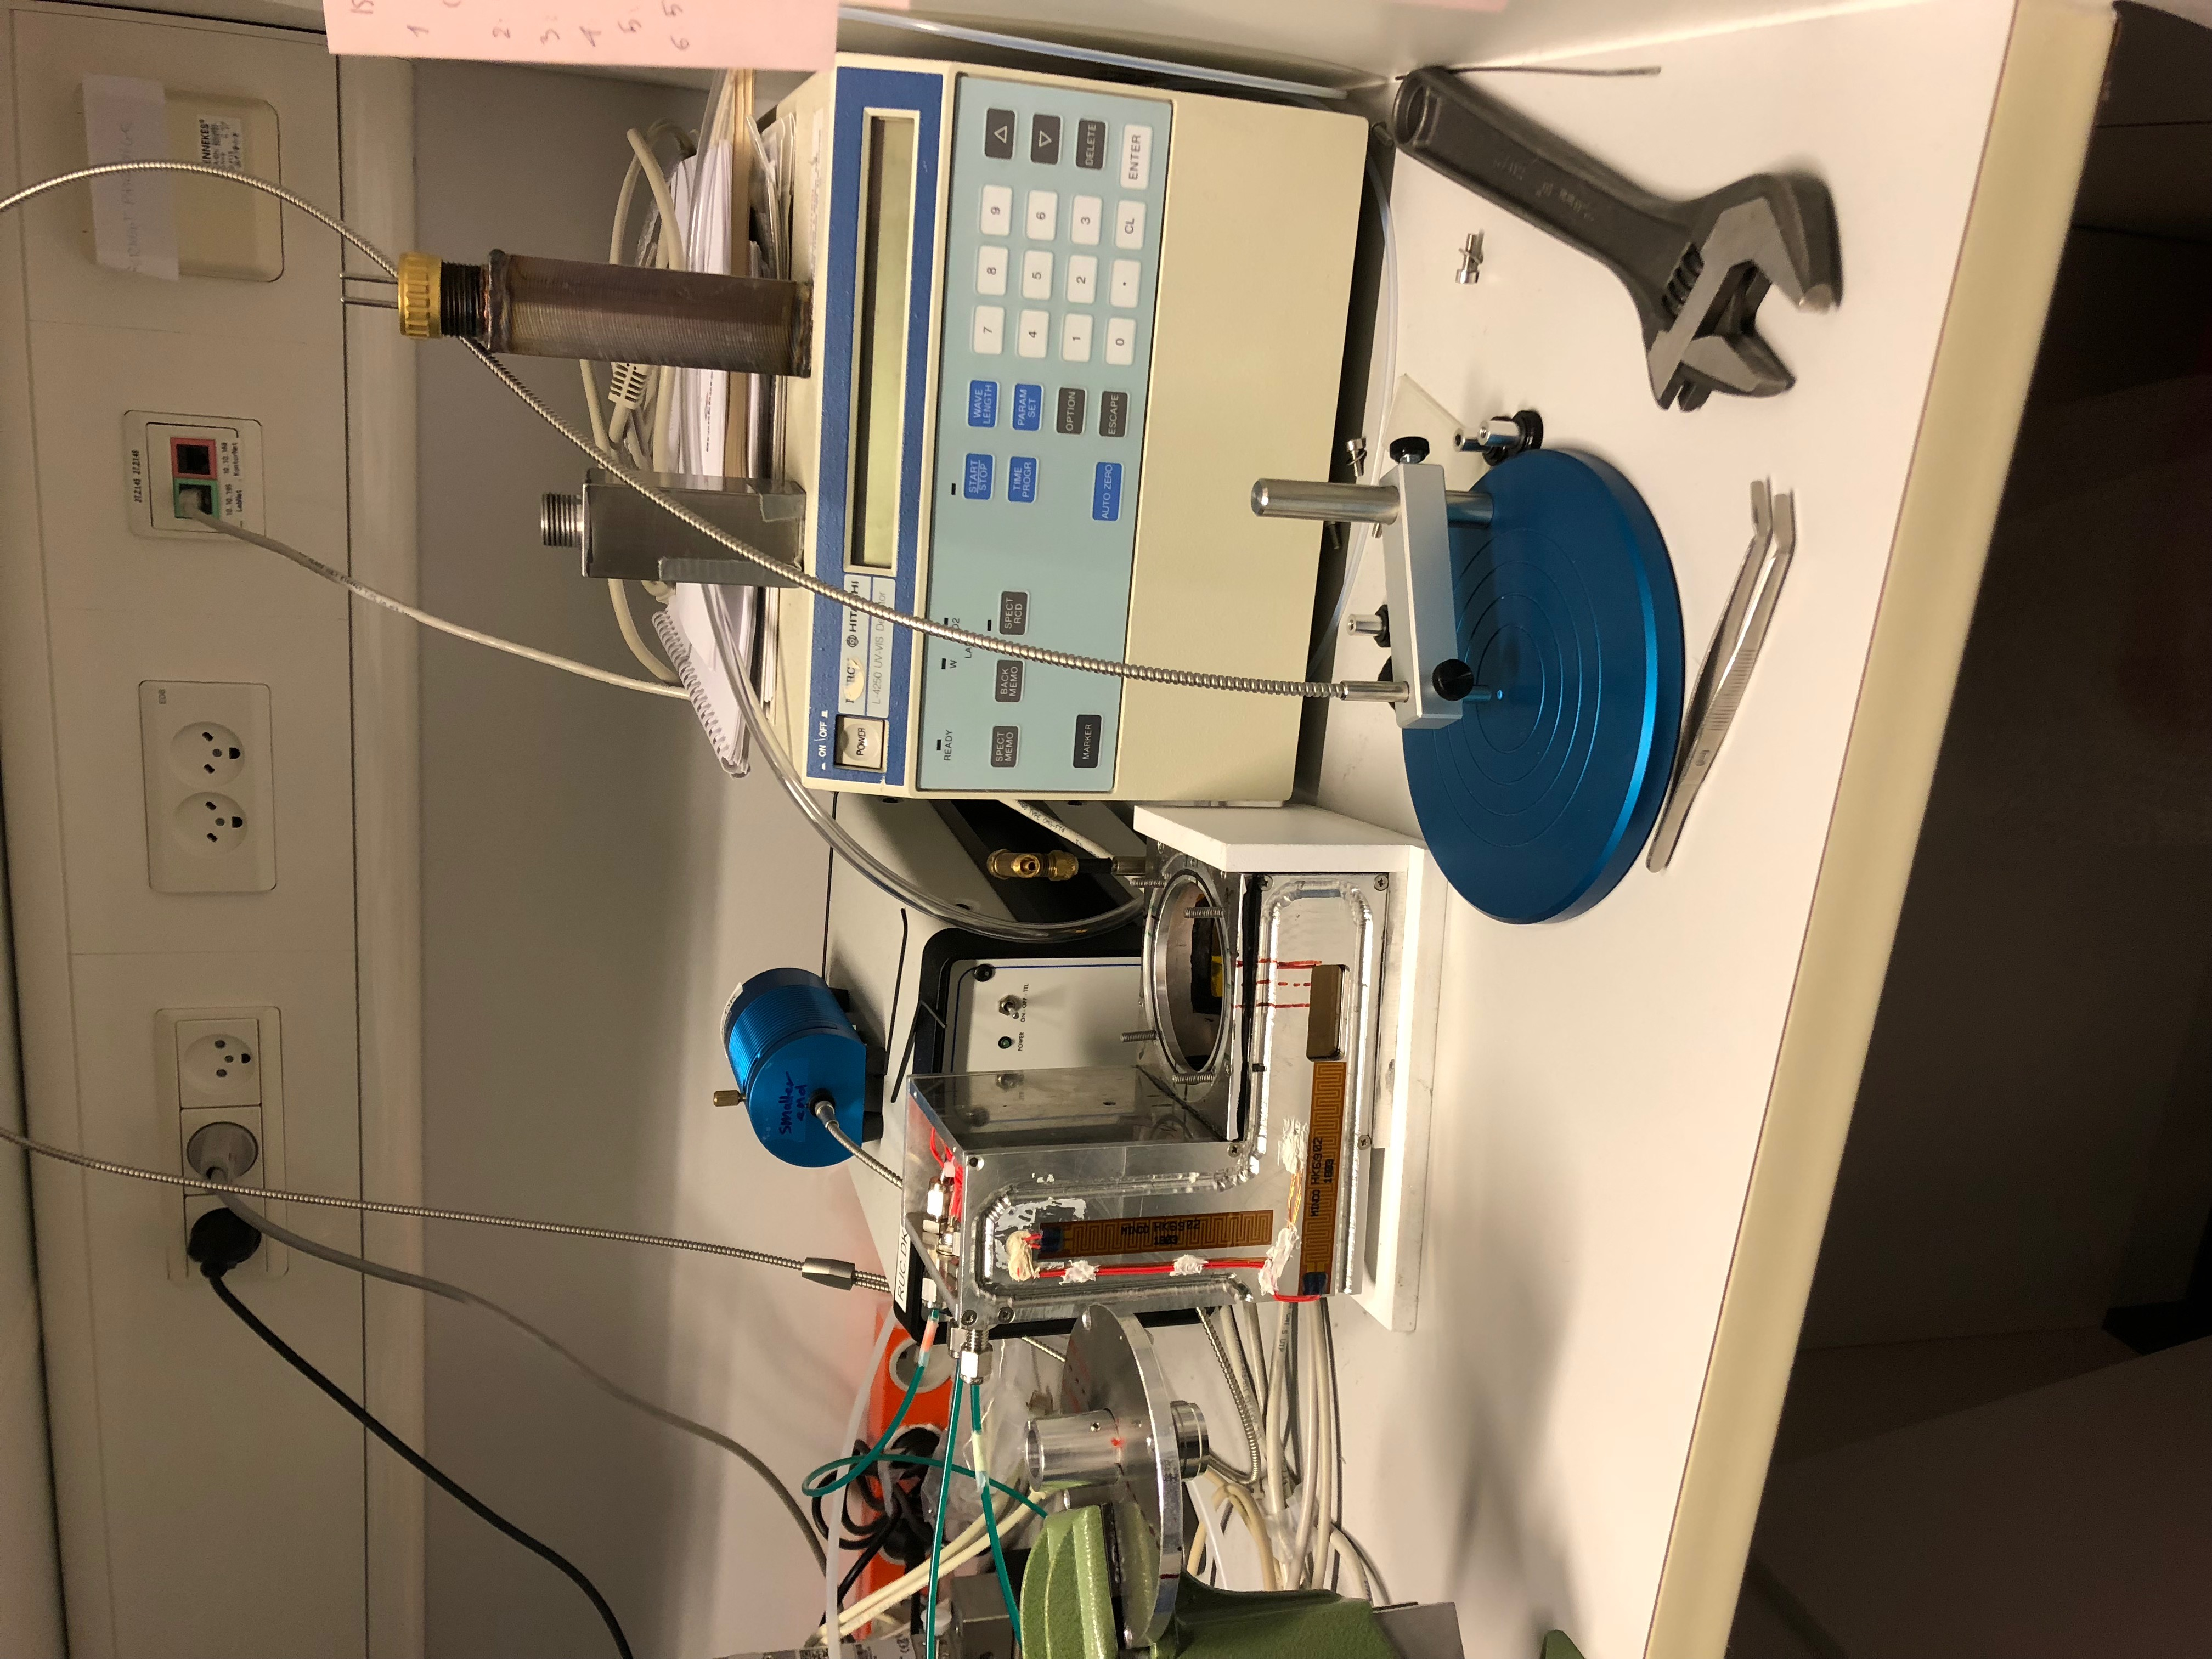
\includegraphics[width=.9\linewidth,angle=-90]{setup1.JPG} 
	    \caption{SVA experiment area}
	    \label{fig:exparea}  
	    \vspace{4ex}
	  \end{minipage}%%
	  \begin{minipage}[b]{0.5\linewidth}
	    \centering
	    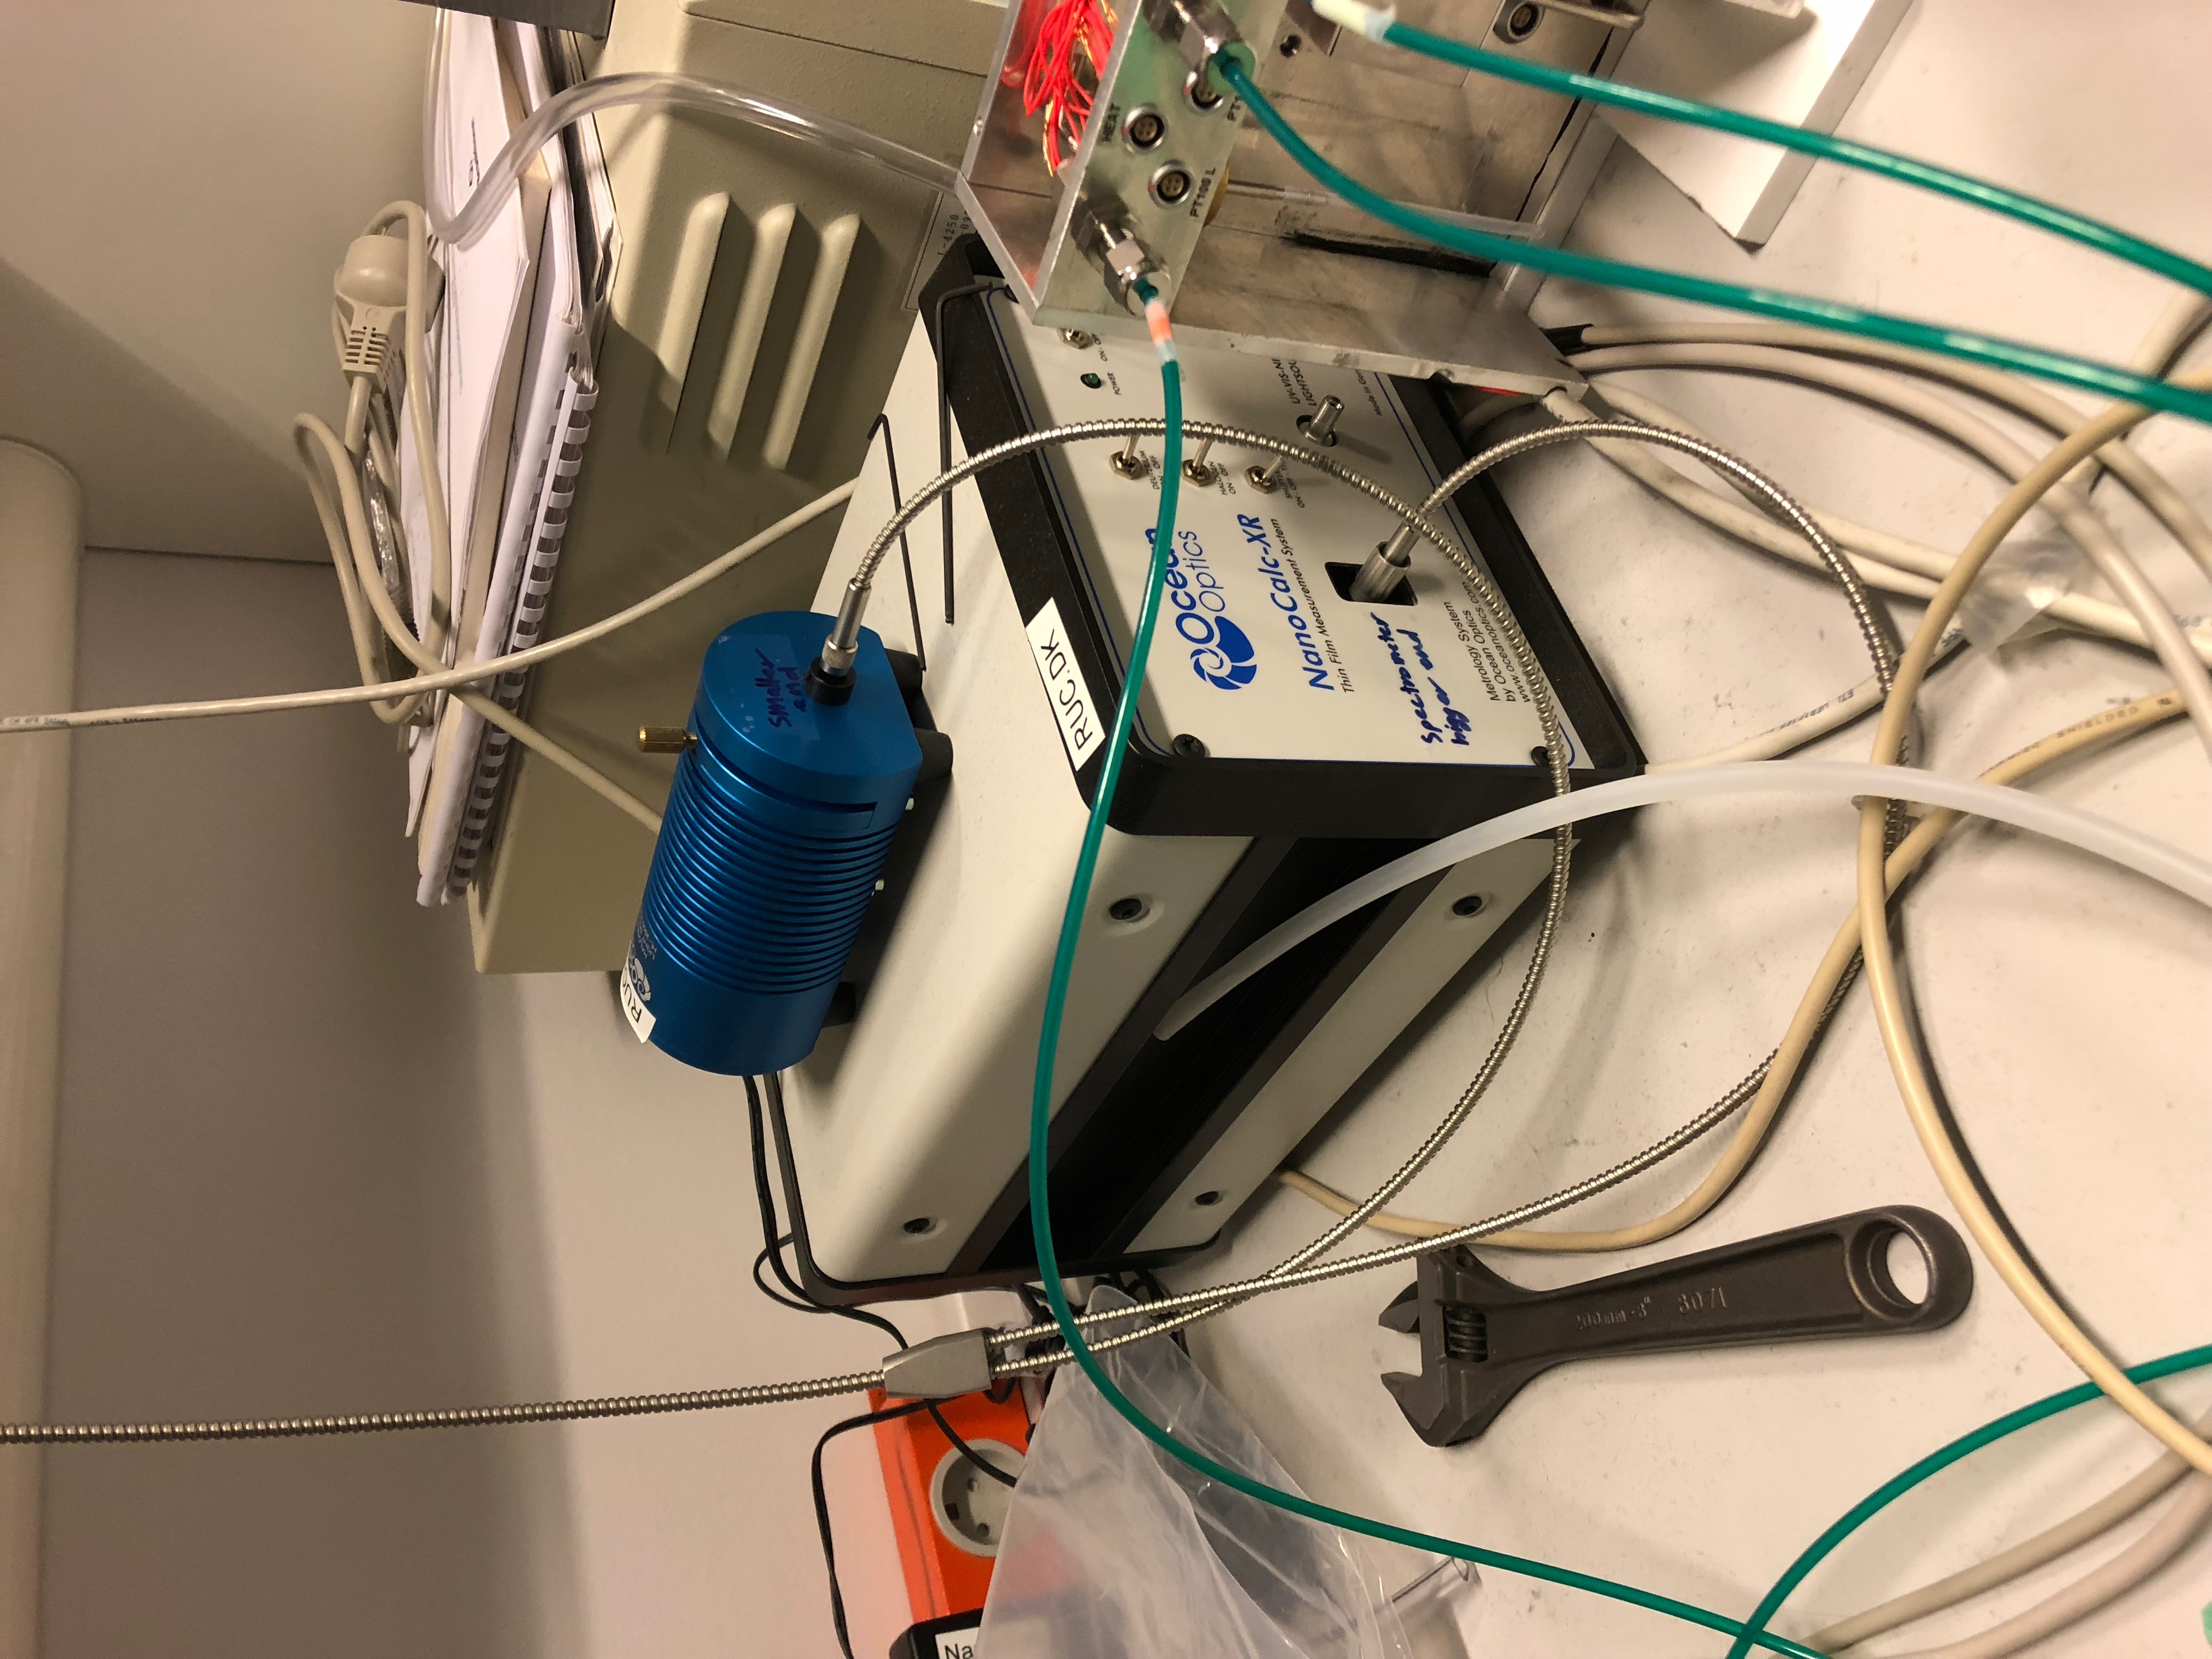
\includegraphics[width=.9\linewidth,angle=-90]{setup2.JPG} 
	    \caption{NanoCalc XR and a Halogen light source(HL-2000-FHSA)}
	    \label{fig:speclight} 
	    \vspace{4ex}
	  \end{minipage} 
	  \begin{minipage}[b]{0.5\linewidth}
	    \centering
	    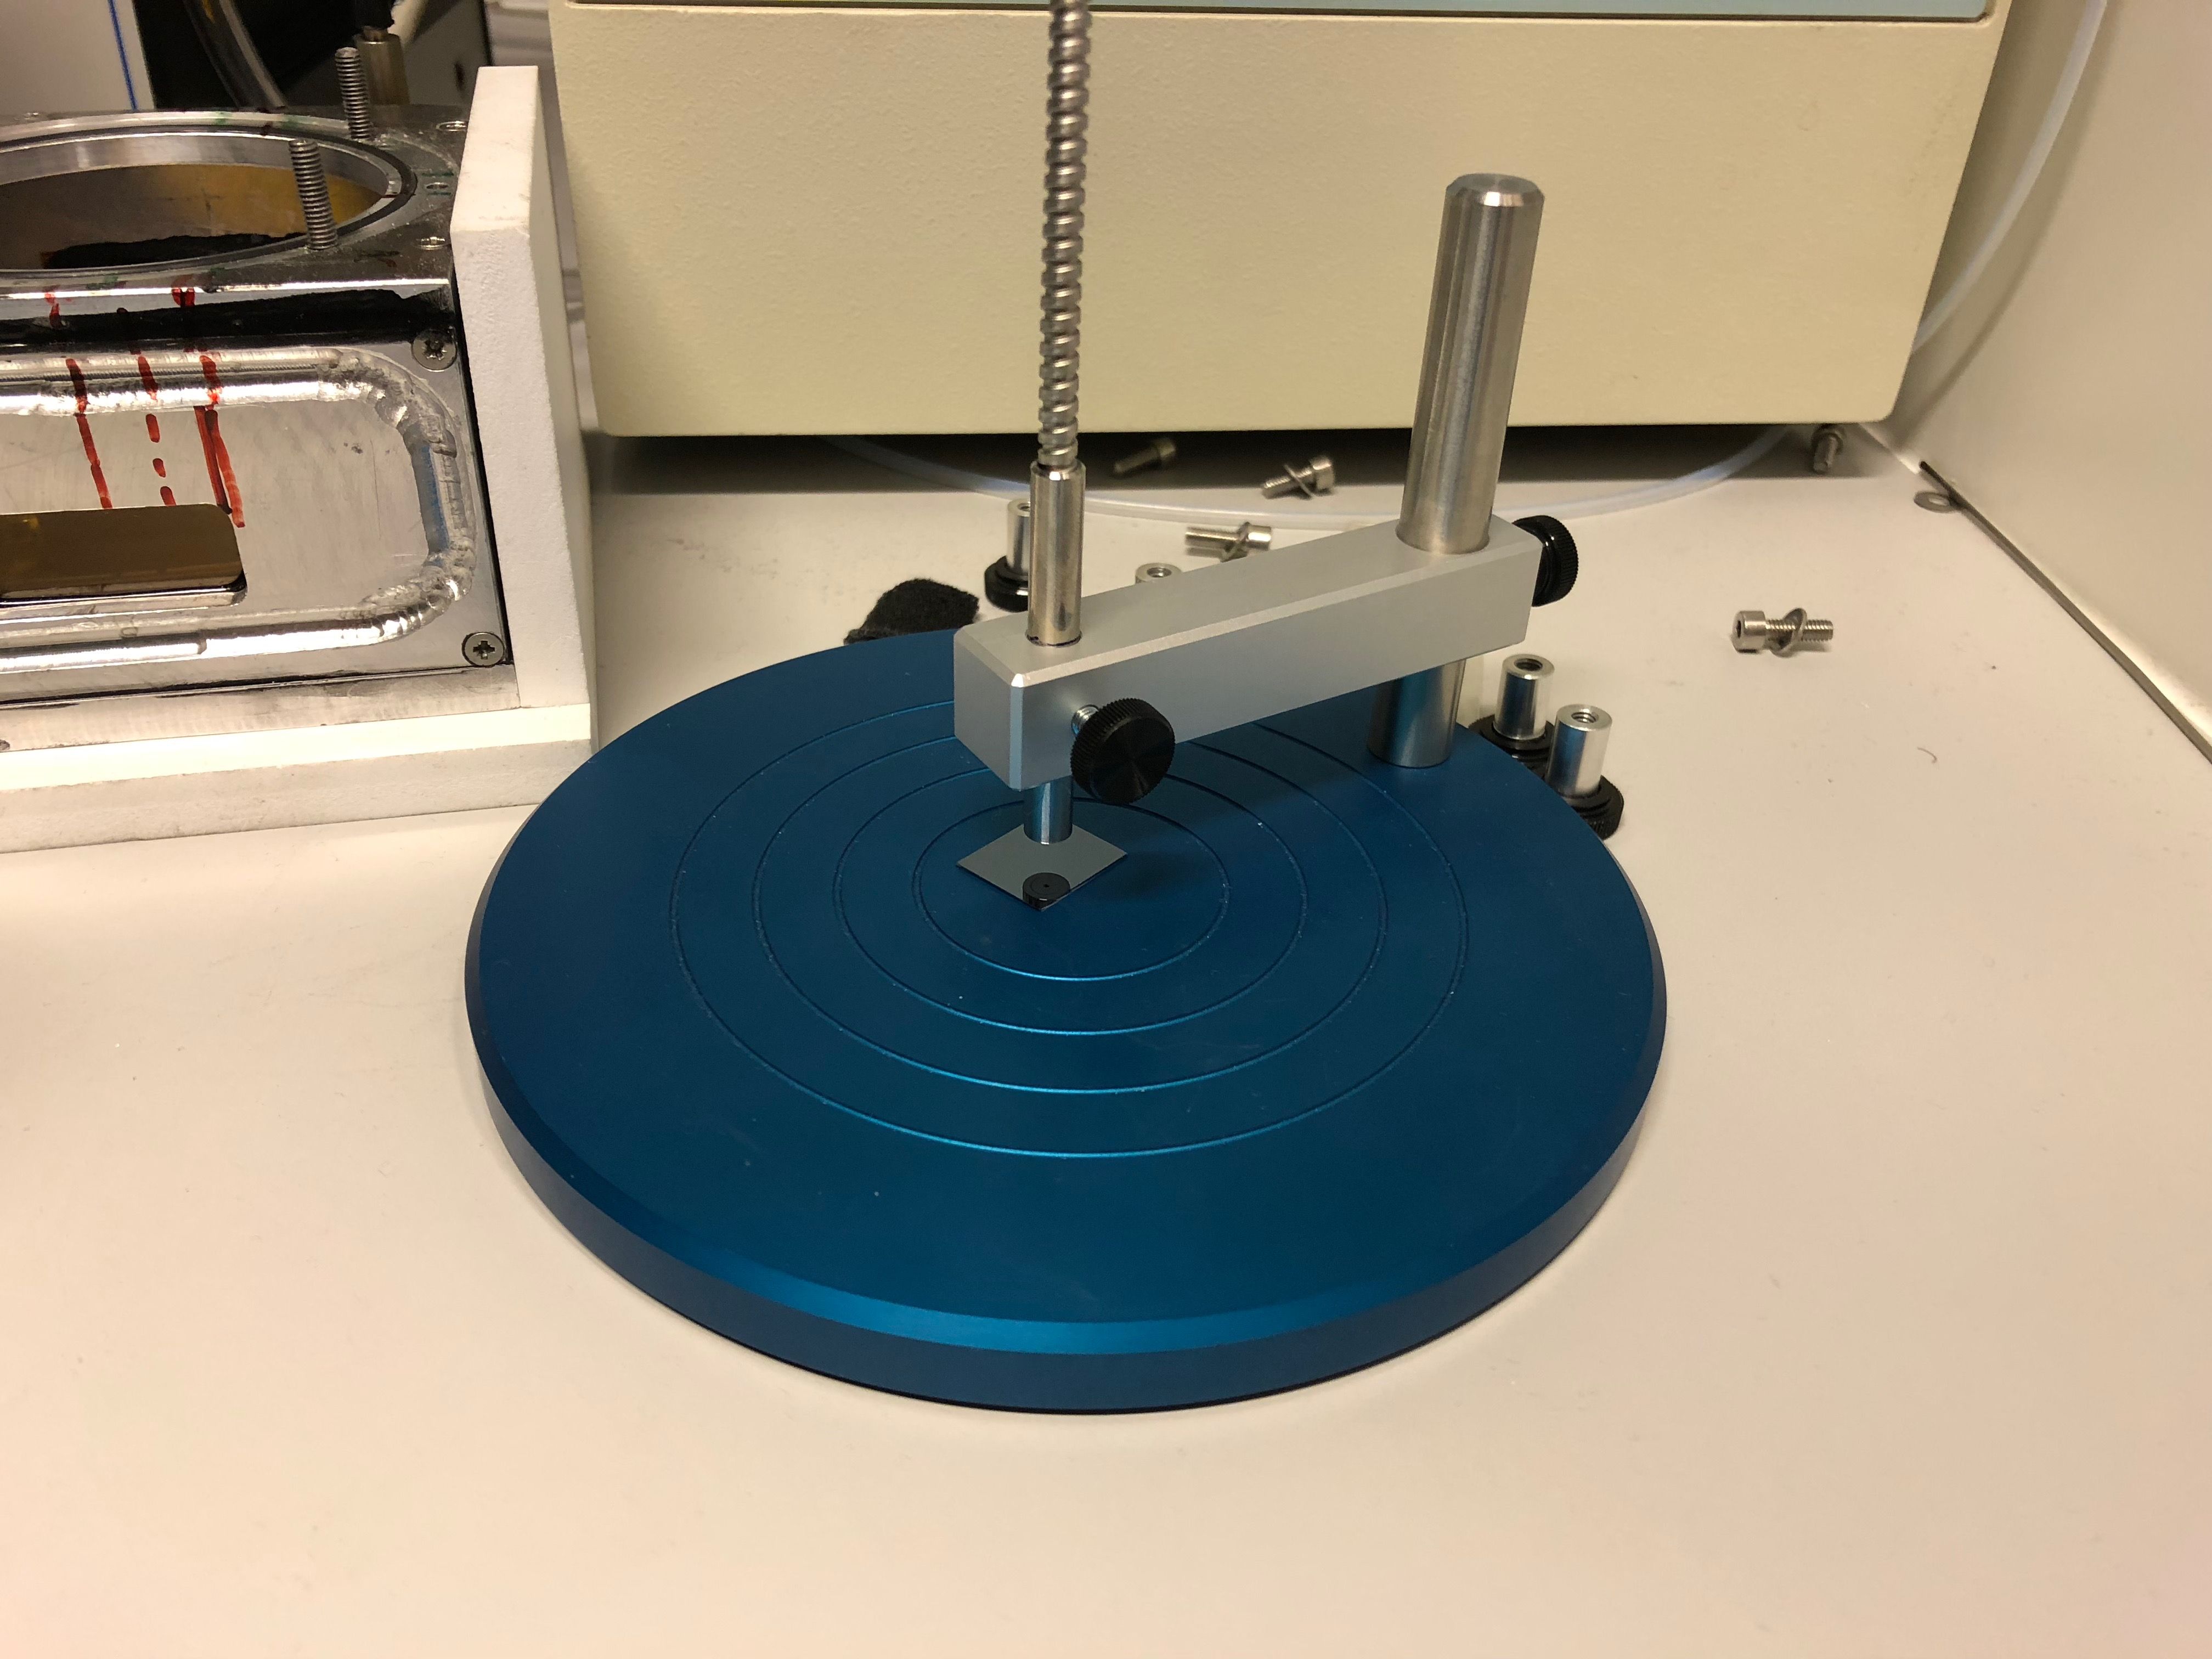
\includegraphics[width=.9\linewidth]{setup3.JPG} 
	    \caption{Single point stage} 
	    \label{fig:Singlestage}
	    \vspace{4ex}
	  \end{minipage}%% 
	  \begin{minipage}[b]{0.5\linewidth}
	    \centering
	    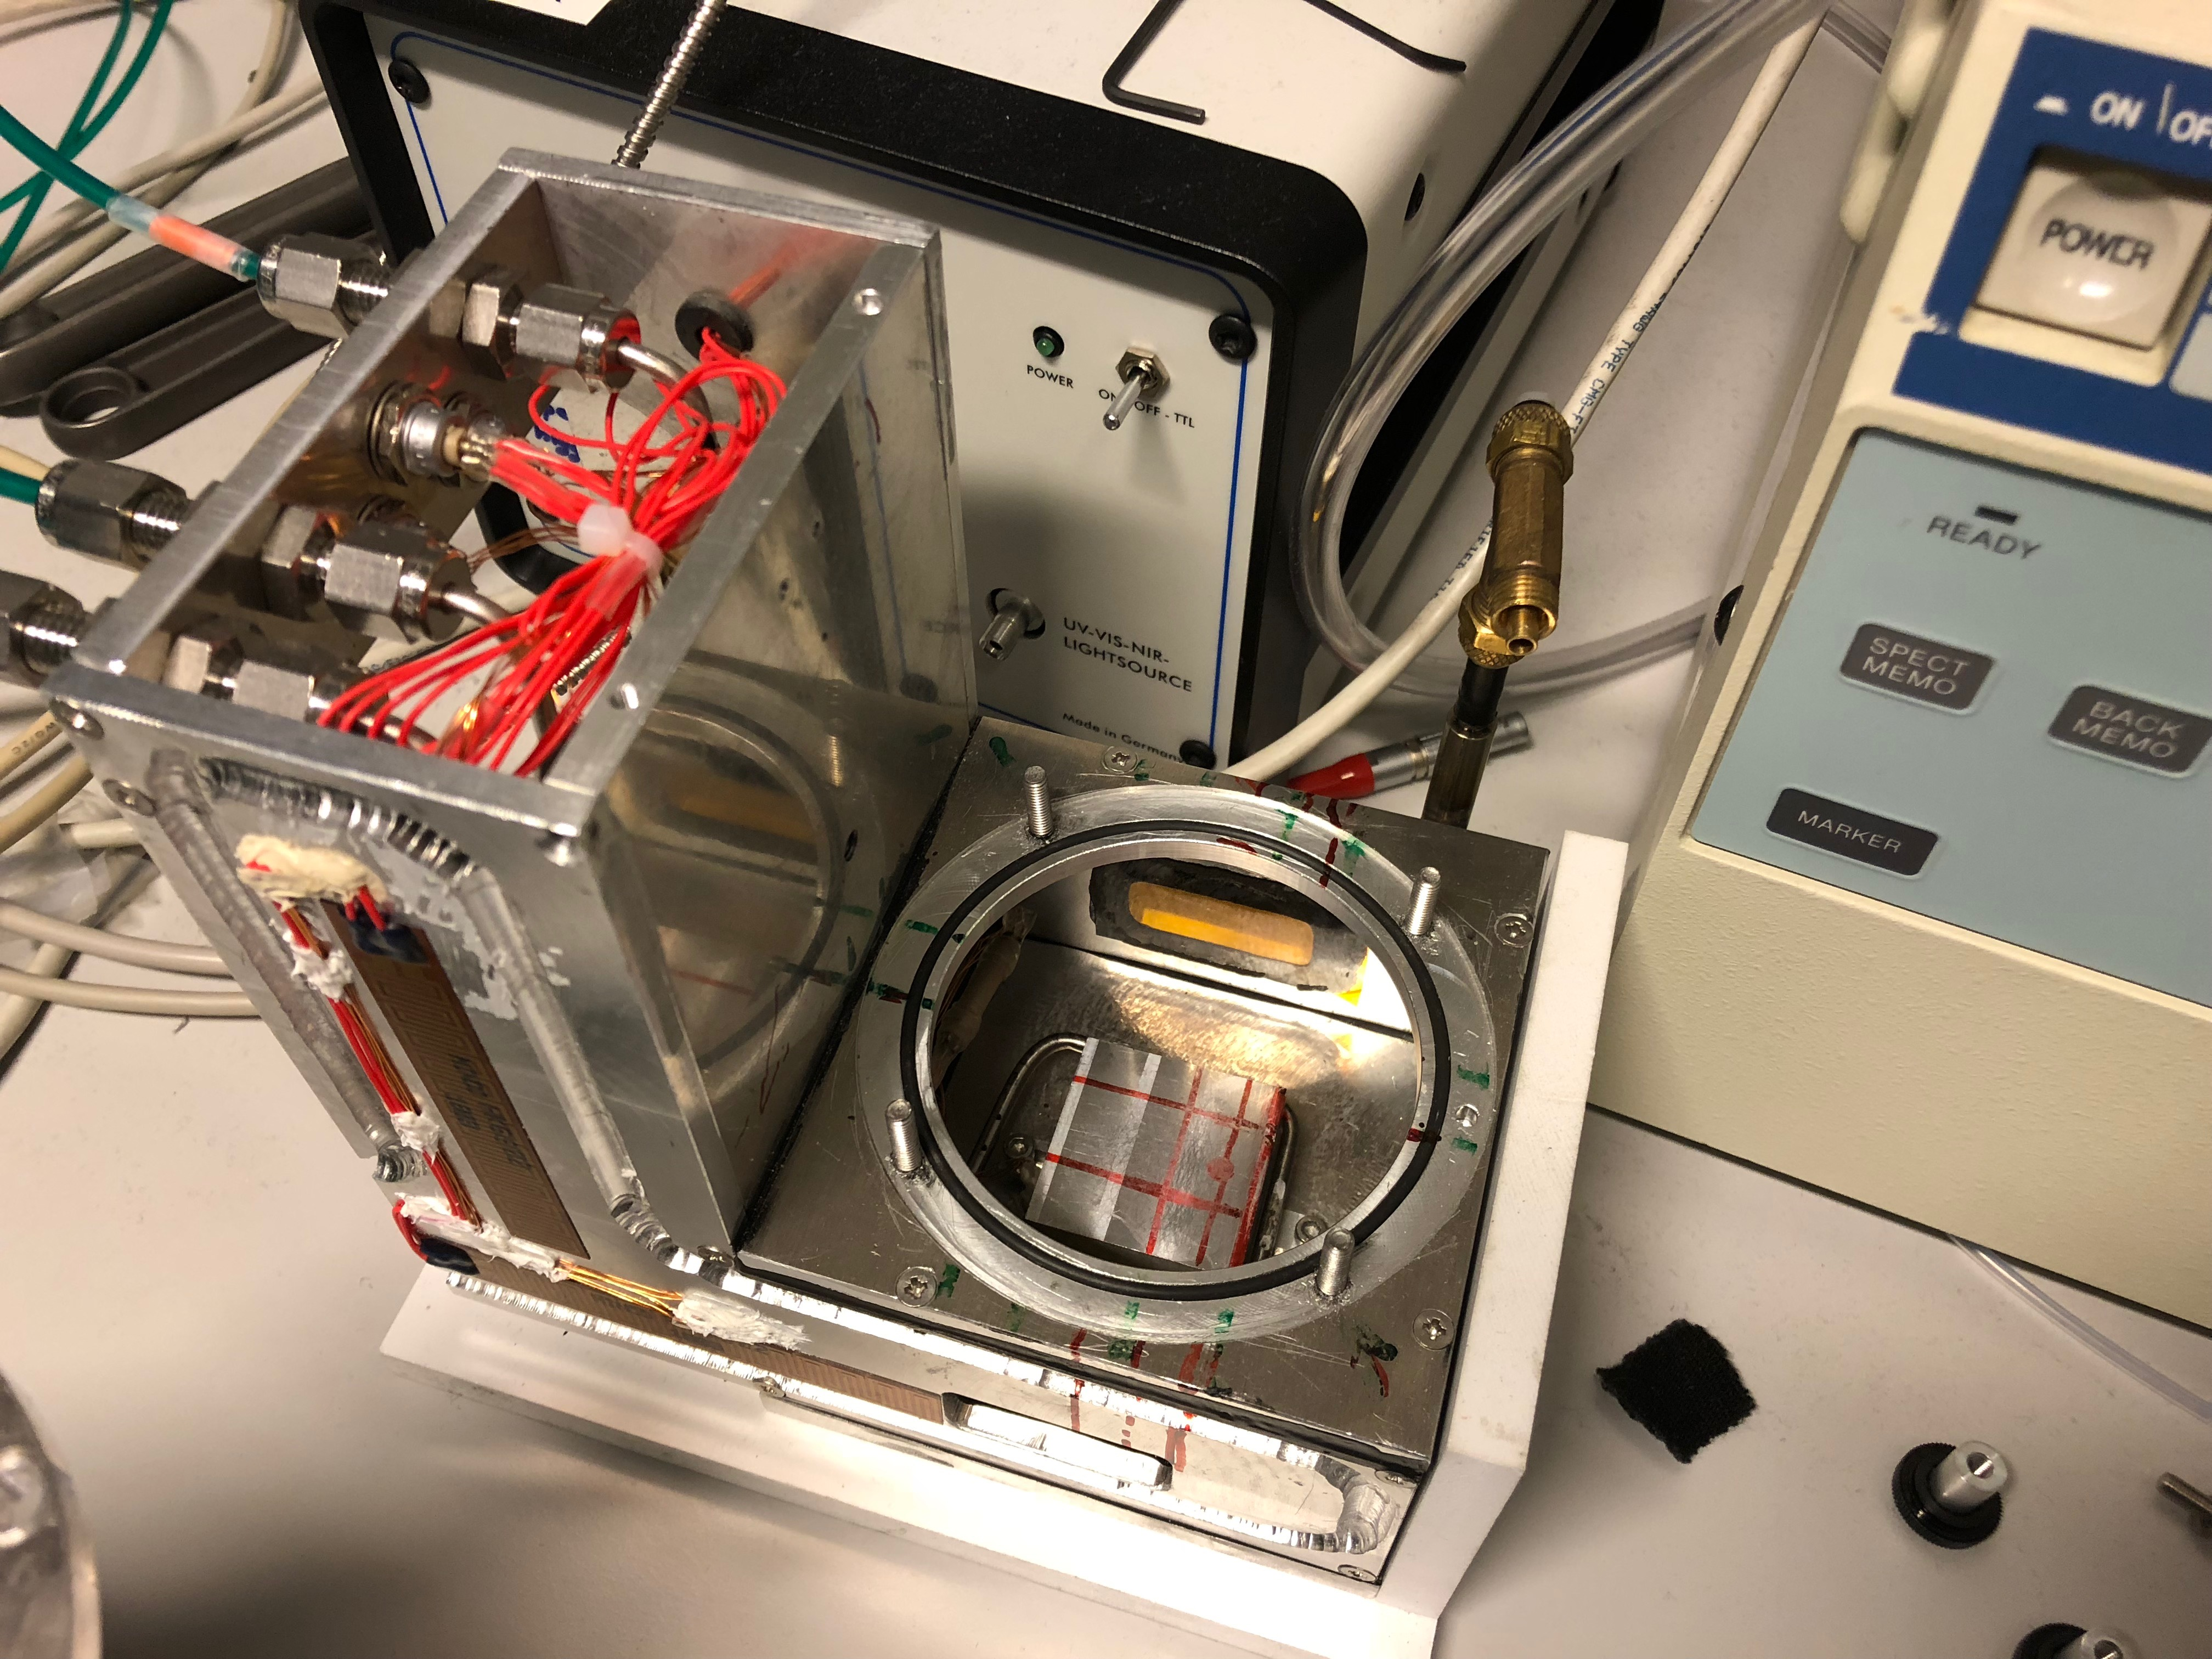
\includegraphics[width=.9\linewidth]{setup4.JPG} 
	    \caption{SVA experiment chamber minus lid}
	    \label{fig:SVAchamber} 
	    \vspace{4ex}
	  \end{minipage} 
	\end{figure}
	
	\begin{figure}
	\centering
		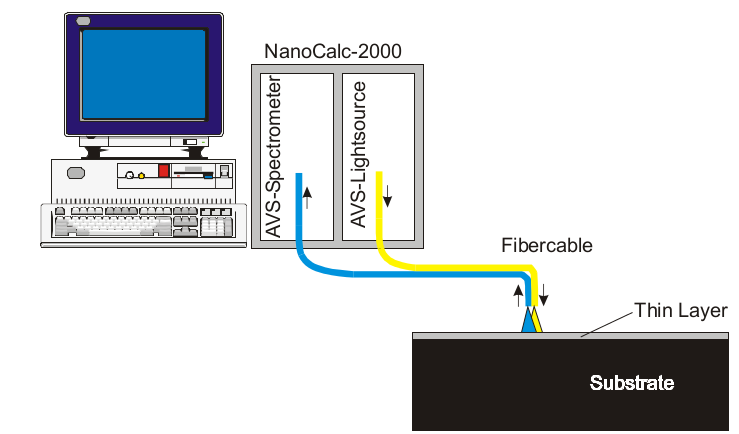
\includegraphics[width=\textwidth]{nanocalcsetup.png}
		\caption{This figure describes the NanoCalc set-up and has been taken from \cite{nanocalcmanual}. Light from a light source travels down the optical fiber illuminating the sample. The reflected light is collected by the optical fiber and analysed in the spectrometer. The spectrometer is connected to the computer by USB and the data is stored, modelled and manipulated through the NanoCalc software.}
		\label{fig:nanocalcsetup}
	\end{figure}
	
\section{Reflectance measurements in the NanoCalc spectrometer}
The NanoCalc spectrometer measures three light intensities which will be called a measurement onwards. The three measurements are the dark measurement (dark), the reference measurement (ref) and the thin-film measurement (meas). The dark measurement is the amount of light received by the optical fiber from external sources. The reference measurement is the amount of light reflected from a blank silicon wafer and the thin film measurement is the amount of light reflected from the sample. From chapter \ref{ch:reflect/trans}, the reflectance of a sample can be expressed as :

\begin{equation}\label{eq:nanocalcrefl}
R_{sample} = \frac{I_{sample}}{I_{incident}}.
\end{equation}

The spectrometer does not measure the intensity of the incident light, therefore the reflectance of the substrate is used to isolate the incident light intensity and inserted into equation \ref{eq:nanocalcrefl}. The reflectance of the substrate is used because it is easily calculated using the Fresnel equations as described in chapter \ref{ch:fresnelref}.

\begin{align}
R_{ref} = \frac{I_{ref}}{I_{incident}}\\
\implies  I_{incident} = \frac{I_{ref}}{R_{ref}} \label{eq:nanocalcrefl2}.
\end{align}

Inserting equation \ref{eq:nanocalcrefl2} in equation \ref{eq:nanocalcrefl}, the reflectance for the sample is expressed without the incident light intensity as:

\begin{equation}
R_{sample} = \frac{I_{sample}}{I_{ref}} \cdot R_{ref}.
\end{equation}

The reflectance of the sample is given as:

\begin{equation}
Reflectance = \frac{Meas-Dark}{Ref-Dark} \cdot R_{sub}.
\end{equation}

This is the same expression given in the NanoCalc spectrometer manual \cite{nanocalcmanual}. Through reproduction of the data and curves given by the NanoCalc spectrometer, i can deduce that the reference measurement has already had the dark measurement subtracted, giving the following reflectance expression:

\begin{equation}\label{eq:nanocalcreflect}
Reflectance = \frac{Meas-Dark}{Ref} \cdot R_{sub}.
\end{equation}

Placing equation \ref{eq:nanocalcreflect} equal to the reflectance equations using the Fresnel equations from chapters  \ref{ch:fresnelref}, \ref{ch:fresnel2lay} and \ref{ch:fresnelmulti}, the NanoCalc spectrometer software can fit a thickness of the sample.


\section{Experimental Protocol}
In this section the experimental protocol for both taking measurements without the optics and with the optics are given. The protocol will be formulated in steps.

\subsection{Without Optics}
\begin{enumerate}
\item Take a continuous reference measurement and adjust the light intensity, such that the reference measurements maximum is $50\%$ of the y-axis.
\item Clear the reference measurement.
\item Take the optic fiber and point it away from anything that can reflect light. Take a dark measurement.
\item Place the optic fiber into ocean optics single point stage. The optic fiber is positioned $4$mm above the single point stage.
\item Place a blank silicon wafer under the optic fiber and take a reference measurement.
\item Save the dark and reference measurement.
\item Place a thin film under the optical fiber and take a measurement.  
\end{enumerate}

\subsection{With Optics}
\begin{enumerate}
\item Take a continuous dark measurement with the optic fiber with a dark cloth in the optics where the thin film would lie and adjust the light intensity, such that the dark measurements maximum is at 100$\%$ of the y-axis.
\item Clear the dark measurement.
\item Take the optics as a whole and point it away from anything that can reflect. Take a dark measurement.
\item Place a blank silicon wafer into the test chamber and place the optics into the test chamber. Take a reference measurement.
\item Save the dark and reference measurement.
\item Take the optics off the test chamber, remove the blank silicon wafer and place in a thin film sample. Place the optics onto the test chamber. Take a measurement.
\end{enumerate}

\section{Solvent Vapour Annealing Process}
\end{document}